\textbf{Цель работы:} изучение вольт-амперной характеристики тлеющего разряда; изучение свойств плазмы методом зондовых характеристик.\\\indent
\textbf{Оборудование:} стеклянная газоразряданя трубка, наполненная неоном, высоковольтный источник питания, источник питания постоянного тока, делитель напряжения, резистор, потенциометр, амперметры, вольтметры, переключатели.

\section*{Теоретические сведения}

\section*{Экспериментальные данные и установка}
\indent Стеклянная газоразрядная трубка имеет холодный полый катод, три анода и геттерный узел — стеклянный баллон, на внутреннюю поверхность которого напылена газопоглощающая плёнка (геттер).
\noindent Катод и один из анодов (I или II) с помощью переключателя П1 подключаются через балластный резистор $R_{\text{б}}$ ($\approx$ 500 кОм) к регулируемому высоковольтному источнику питания (ВИП) с выходным напряжением до нескольких киловольт.
\indent При подключении к ВИП анода-I между ним и катодом возникает газовый разряд.
Ток разряда измеряется миллиамперметром A1, а падение напряжения на разрядной трубке — вольтметром V1.
При подключении к ВИП анода-II разряд возникает в пространстве
между катодом и анодом-II, где находится двойной зонд, используемый для диагностики плазмы положительного столба.
Зонды изготовлены
из молибденовой проволоки диаметром d = 2  мм и имеют длину l = 5.2 мм. Они подключены к источнику питания через потенциометр R. Переключатель П2 позволяет изменять полярность напряжения на зондах.
Для измерения зондового тока используется
микроамперметр A2. Анод-III в нашей работе не используется.
\begin{figure}[h!]
    \centering
    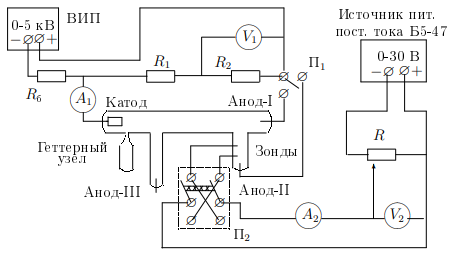
\includegraphics[width=10cm]{setup.png}
    \caption{Cхема экспериментальнoй установки}
\end{figure}
\newpage
\subsection*{Вольт-ампераня характеристика разряда}
Определим напряжение зажигания разряда $U_{\text{разр}} = 200$ В.
\begin{table}[h!]
    \centering
    \begin{tabular}{|c|c|c|c|c|c|c|c|c|c|c|c|c|}
        \hline
        $I$, мА & 0.52& 0.80& 1.13& 1.439& 1.84& 2.42& 2.98& 3.33& 3.87& 4.45& 2.13& 1.65 \\\hline
        $U$, В & 34.3& 32.9& 32.1& 31.5& 27.8& 21.4& 18.3& 16.9& 15.9& 15.3& 23.6& 30.3\\\hline
    \end{tabular}
    \caption{ВАХ разряда при нарастании тока}
\end{table}

\begin{table}[h!]
    \centering
    \begin{tabular}{|c|c|c|c|c|c|c|c|c|c|c|}
        \hline
        $I$, мА & 4.721& 4.31& 3.939& 3.570& 3.203& 2.827& 2.469& 1.852& 1.100& 0.594\\\hline
        $U$, В & 14.9& 15.4& 15.8& 16.2& 17.3& 19.1& 21.0& 23.3& 32.1& 33.8\\\hline
    \end{tabular}
    \caption{ВАХ разряда при убывании тока}
\end{table}
\begin{figure}[h!]
    \centering
    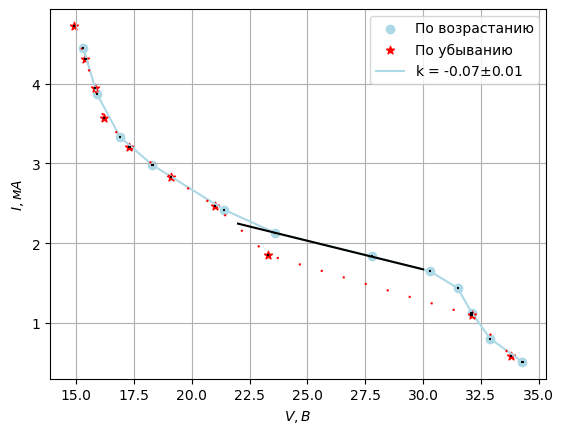
\includegraphics[width=12cm]{images/plot1.png}
    \caption{ВАХ разряда при убывании и нарастании тока}
\end{figure}

Из графика находим $R_{\text{диф}}^{\text{max}} = \frac{dU}{dI} = (13.98 \pm 0.05)\cdot 10^{3}$ Ом

\subsection*{Зондовые характеристики}
Установим разрядный ток $I_{\text{р}} = 5$ мА. И снимем вольт-амперную характеристику двойного зонда. По полученным графикам определим температуру электронов по формуле:
\begin{equation}
    kT_e = \frac{1}{2}\frac{eI_{\text{iн}}}{\frac{dI}{dU}\vline_{U=0}}
\end{equation}
\begin{table}[h!]
    \centering
    \begin{tabular}{|c|c|c|c|c|}
        $I_{\text{р}}$, мА
    \end{tabular}
\end{table}


\newpage
\begin{table}[h!]
    \centering
    \begin{tabular}{|c|c|c|c|c|c|c|c|c|c|c|c|c|c|}
        \hline
        \multirow{2}{*}{$I_{\text{р}} = 5$ мА} & $I$, мА & 82.5&85.9&84.7&81.5&74.6&62.4&50.6&36.5&19.9&-24.4&-42.5&-51.9\\
        &$U$, В & 25.01&  22.03&  19.  &  16.04&  13.03&  10.04&   8.01&   6.02& 4.03&  -2.02&  -4.08&  -6.01\\\hline
        \multirow{2}{*}{$I_{\text{р}} = 4$ мА} & $I$, мА & 70.6&  70.3&  68.5&  65.7&  60.6&  51.1&  42.3&  30.5&  17.1&
       -23.5& -38.9& -51.5\\
       &$U$, В & 25.03& 22.08& 19.04& 16.  & 13.04& 10.02&  8.06&  6.07&  4.01&
       -2.04& -4.06& -6.06\\\hline
       \multirow{2}{*}{$I_{\text{р}} = 3$ мА} & $I$, мА & 52.6 &  50.9 &  49.17&  47.2 &  44.  &  38.1 &  32.02&  23.5 &
        13.5 & -20.3 & -31.5 & -41.0\\
       &$U$, В & 25.03& 22.04& 19.03& 16.06& 13.04& 10.03&  8.07&  6.  &  4.03&
       -2.03& -4.08& -6.08\\\hline
       \multirow{2}{*}{$I_{\text{р}} = 1.5$ мА} & $I$, мА & 24.6&  23.8&  23. &  22.2&  21.1&  18.8&  16.1&  12.2&   7.1&
       -12.3& -17.9& -22.7\\
       &$U$, В & 25.  & 22.09& 19.06& 16.03& 13.08& 10.06&  8.05&  6.04&  4.09&
       -2.17& -4.06& -6.02\\\hline
    \end{tabular}
    \caption{ВАХ двойного зонда при различных токах разряда}
\end{table}
\begin{figure}[h!]
    \centering
    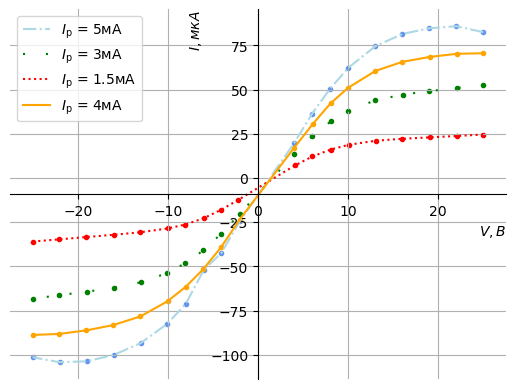
\includegraphics[width=15cm]{images/plot2.png}
    \caption{Сравнение ВАХ двойного зонда при различных токах разряда}
\end{figure}

\newpage

\begin{figure}[h!]
    \begin{subfigure}{0.5\linewidth}
        \centering
        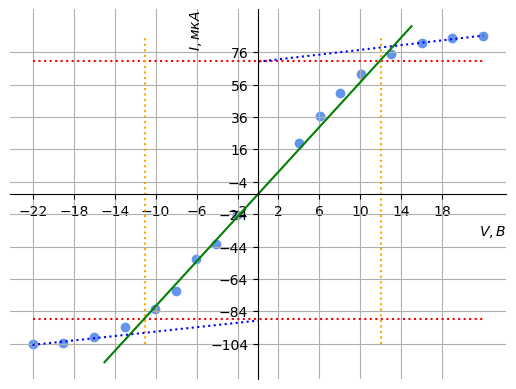
\includegraphics[width=10cm]{images/plotI_5.png}
        \caption{При $I_{\text{р}}$ = 5 мА}
    \end{subfigure}
    \hfill
    \begin{subfigure}{0.5\linewidth}
        \centering
        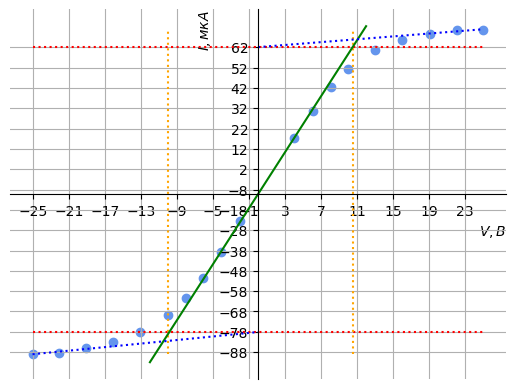
\includegraphics[width=10cm]{images/plotI_4.png}
        \caption{При $I_{\text{р}}$ = 4 мА}
    \end{subfigure}
    \vfill
    \begin{subfigure}{0.5\linewidth}
        \centering
        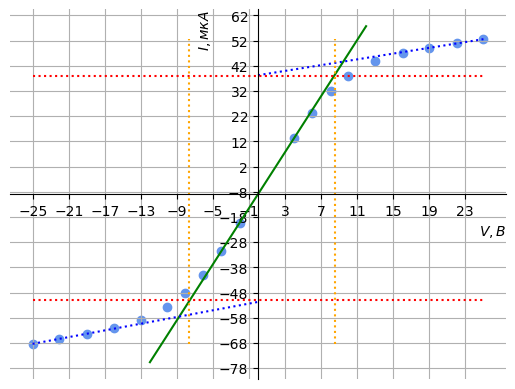
\includegraphics[width=10cm]{images/plotI_3.png}
        \caption{При $I_{\text{р}}$ = 3 мА}
    \end{subfigure}
    \hfill
    \begin{subfigure}{0.5\linewidth}
        \centering
        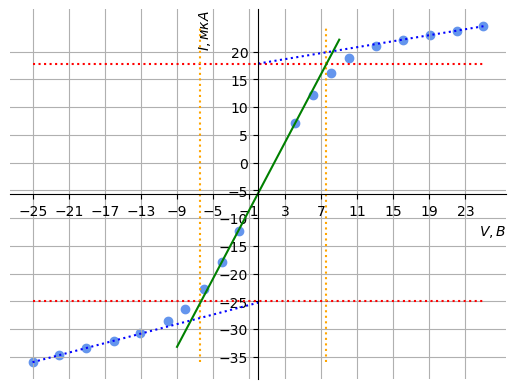
\includegraphics[width=10cm]{images/plotI_1.5.png}
        \caption{При $I_{\text{р}}$ = 1.5 мА}
    \end{subfigure}
    \caption{ВАХ двойного зонда при различных значениях тока разряда $I_{\text{р}}$}
\end{figure}


